% EPC flow charts
% Author: Fabian Schuh
\documentclass{article}
\usepackage{myflowchart}

\begin{document}
\begin{tikzpicture}

\begin{scope}[node distance=5mm and 5mm]

\node [ item=4](a) at (1,1) {%
            \textbf{可預測、必要的連結步驟}
            \nodepart{two}
            \begin{enumerate}
            	\item Read old notes, review, add, adjust, or collect
            	\item watch CS matches
            	\item 理髮刮鬍
            	\item git comment, push(github現在很難連上), 備份
            	\item git read, try new functions, apply
            	\item 採買(修理零件,烘焙食物,早餐)
           \end{enumerate}
           \nodepart{three}\textbf{持續性}
	\nodepart{four}
            \begin{enumerate}
            	\item 尋找工作地點
           \end{enumerate}
            };

\node [above right = of a, align = center, anchor = south] (title){
\parbox[c][][c]{0.3\textwidth}{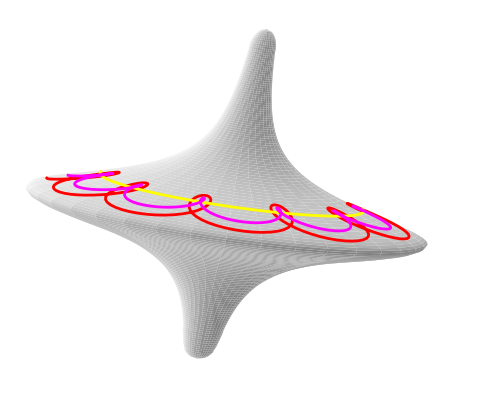
\includegraphics[width=0.3\textwidth]{../../figs/logo_June27_2016.png}}\parbox[c][][c]{5cm}{\Huge Connectors\\Splices\\Chores}
 };

\node [ item=2, below right = of title.south, anchor = north west](small) {%
            \textbf{不可預測、必要的連結步驟}
            \nodepart{two}
            \begin{enumerate}
            	\item 洗米煮米。
            	\item 煮飯或買菜。老媽有時候不會煮飯或買菜,這一點完全無法預測,變成這件事情是會臨時出現而打亂其他行程,非常麻煩。
		\item 兩個禮拜就要花時間30分鐘清理冰箱,包括丟掉過期的,然後洗盒子,整理未過期的(將剩菜裝進盒子,因為全部都用袋子非常亂也浪費),每三天要洗一次電鍋。每兩天就要洗米煮米。
		\item 早上第一件事情就是罵人,導致心情鬱卒,胸口鬱悶,做事出錯率變高,也是很麻煩,變成一件事情需要兩三倍時間才能完成,也沒辦法。這兩件事看有無辦法提升效率。
           \end{enumerate}
            };

\end{scope}
\end{tikzpicture}
\end{document}
